\documentclass[11pt,a4paper,twoside]{article}

% Input encoding and basic packages
\usepackage[utf8]{inputenc}
\usepackage{amsmath, amssymb}
\usepackage{graphicx}
\usepackage{tcolorbox}
\usepackage{xcolor}
\usepackage{geometry}
\usepackage{wrapfig}
\usepackage{titlesec}
\usepackage{fancyhdr}
\usepackage{caption}
\usepackage{float}
\usepackage{hyperref}
\usepackage{subcaption}
\usepackage{fontspec}
\usepackage{nomencl} 
\usepackage{multicol}
\usepackage{etoolbox}
\usepackage{sectsty} % Allows custom section styles
\usepackage{helvet}  % Default sans-serif font
\usepackage{times}   % Example serif font for body text

% Define custom fonts
\setmainfont{Poppins} % Main font for body text
\newfontfamily\titlesfont{Anonymous Pro} % Font for titles

% Relax Latex rules for text layout
\raggedbottom
\sloppy
\hbadness=10000

% Define custom colors
\definecolor{cherenkovblue}{RGB}{55, 139, 230}

% Adjust default font sizes (Explicitly set sizes)
\renewcommand{\normalsize}{\fontsize{9}{11}\selectfont} % Smaller body text: 9pt font with 11pt line spacing
\renewcommand{\small}{\fontsize{8}{10}\selectfont}
\renewcommand{\footnotesize}{\fontsize{7}{9}\selectfont}

% Make titles all caps
\makeatletter
\let\oldsection\section
\renewcommand{\section}{\@startsection {section}{1}{\z@}%
  {-3.5ex \@plus -1ex \@minus -.2ex}%
  {2.3ex \@plus.2ex}%
  {\titlesfont\fontsize{14}{16}\bfseries\color{cherenkovblue}\MakeUppercase}}
\makeatother

% Custom subsection font
\subsectionfont{\titlesfont\fontsize{12}{14}\bfseries\color{cherenkovblue}} % Subsection: 12pt font, bold, blue

% Customize spacing
\setlength{\parskip}{6pt} % Add spacing between paragraphs
\setlength{\parindent}{0pt} % Remove paragraph indentation
\setlength{\itemsep}{4pt} % Add spacing between list items

% Customize itemize bullets
\renewcommand\labelitemi{--} % Use dashes instead of bullets

% Define fancy header and footer
\fancypagestyle{plain}{
    \fancyhf{} % Clear all header and footer fields
} % Default plain style for title and index pages

\fancypagestyle{post-index}{
    \fancyhf{} % Clear all header and footer fields
    \fancyhead[LE]{\textit{S.Pagliuca, T.Pirola, L.Raffuzzi, R.Ronchi, D.Shabi}}
    \fancyhead[RO]{\textit{Nuclear Design and Technologies}}
    \fancyfoot[LE,RO]{\thepage}
    \renewcommand{\headrulewidth}{0.4pt}
    \renewcommand{\footrulewidth}{0.4pt}
    \setlength{\headheight}{14pt}
}

\begin{document}
%%%%%%%%%%%%%%%%%%%%%%%%%%%%%%%%%%%%%%%%%%%%%%%%%%%%%%%%%%%%%%%%%%%%%%%%%%%%%%%%%%%%%%%%%%%%
% First page
% Includes title, author, abstract, keywords, nomenclature
\thispagestyle{plain}

% Title with Titles Font (Anonymous Pro)
{\titlesfont\fontsize{18}{28}\textbf{\color{cherenkovblue}{FUEL PIN \\ PRELIMINARY DESIGN}}}\\
{\titlesfont\fontsize{10}{12}\color{cherenkovblue} Nuclear Engineering - Politecnico di Milano}\\


\vspace{-10pt}

% Author information with Main Font (Poppins)
{\normalsize\textbf{Simone Pagliuca, Tommaso Pirola, Lisa Raffuzzi, Riccardo Ronchi, Darien Shabi}} \\
{\footnotesize\textit{simone1.pagliuca@mail.polimi.it}} \\

\vspace{10pt}

% Course and Academic Year
{\footnotesize\textbf{Course:} Nuclear Design and Technologies}\\
{\footnotesize\textbf{Academic year:} 2024/2025}

% Horizontal rule
\vspace{8pt}
\centerline{\rule{1.0\textwidth}{0.4pt}}

\vspace{10pt}

% Abstract with Titles Font for Heading, Main Font for Body
{\fontsize{8}{8}\textbf{\color{cherenkovblue} ABSTRACT:}} 
{\normalsize
    lorem ipsum dolor sit amet, consectetur adipiscing elit. Donec auctor, nunc nec ultricies ultricies, nunc nunc.
}

\vspace{10pt}

% Key-words box with Titles Font
\begin{tcolorbox}[arc=0pt, boxrule=0pt, colback=cherenkovblue!60, width=\textwidth, colupper=white]
    {\titlesfont\fontsize{10}{10}\textbf{Key-words:}} Key, Words, Here
\end{tcolorbox}

\vspace{10pt}

% Nomenclature Definitions
\makenomenclature
\renewcommand\nomgroup[1]{%
\item[\bfseries
\ifstrequal{#1}{A}{A Quantities}{%
\ifstrequal{#1}{B}{B Quantities}{}}%
]}

% Two-column layout for the nomenclature
\renewcommand{\nompreamble}{\begin{multicols}{2}}
\renewcommand{\nompostamble}{\end{multicols}}

% Define Nomenclature Entries
\nomenclature[A, 01]{$x$}{X quantity}
\nomenclature[B]{$y$}{Y quantity}

% Render Nomenclature Without Section Break
\vspace{-5pt} % Adjust spacing to fit table
\printnomenclature

\newpage
%%%%%%%%%%%%%%%%%%%%%%%%%%%%%%%%%%%%%%%%%%%%%%%%%%%%%%%%%%%%%%%%%%%%%%%%%%%%%%%%%%%%%%%%%%%%

%%%%%%%%%%%%%%%%%%%%%%%%%%%%%%%%%%%%%%%%%%%%%%%%%%%%%%%%%%%%%%%%%%%%%%%%%%%%%%%%%%%%%%%%%%%%
% Table of contents
% Switches to the post-index page style after TOC
\tableofcontents
\newpage
\pagestyle{post-index}
%%%%%%%%%%%%%%%%%%%%%%%%%%%%%%%%%%%%%%%%%%%%%%%%%%%%%%%%%%%%%%%%%%%%%%%%%%%%%%%%%%%%%%%%%%%%

%%%%%%%%%%%%%%%%%%%%%%%%%%%%%%%%%%%%%%%%%%%%%%%%%%%%%%%%%%%%%%%%%%%%%%%%%%%%%%%%%%%%%%%%%%%%
\section{Introduction}
The fuel pin design process involves:
\begin{itemize}
    \item Determining the cladding thickness, the fuel-cladding gap size, and the plenum height.
    \item Verifying the design against limits for fuel melting, cladding temperature, yielding, and thermal creep.
    \item Identifying critical aspects if the irradiation time is doubled.
\end{itemize}
Most design specifications were provided. Missing data were sourced from literature or handouts. 


%%%%%%%%%%%%%%%%%%%%%%%%%%%%%%%%%%%%%%%%%%%%%%%%%%%%%%%%%%%%%%%%%%%%%%%%%%%%%%%%%%%%%%%%%%%%
\section{Assumptions and Methodology}
\subsection{Material and Thermal Assumptions}
\begin{itemize}
    \item Axial profiles for power and neutron flux were assumed constant in time.
    \item Initial helium pressure and temperature in the fuel-cladding gap were taken as specified.
\end{itemize}

\begin{figure}[H]
    \centering
    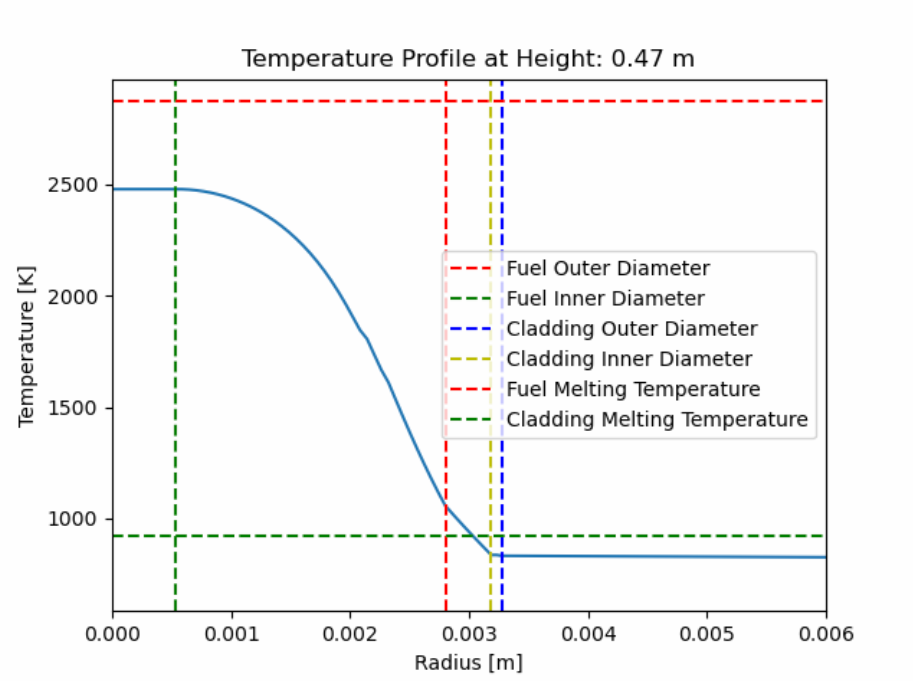
\includegraphics[width=0.8\textwidth]{temperature_profile.png}
    \caption{Radial temperature profile within the fuel pin. The profile shows the temperature distribution at the middle node.}
    \label{fig:Temperature_Profile}
\end{figure}

\subsection{Fission Gas Release Model}
\begin{itemize}
    \item \textbf{Domain size:} Grain size $d_g = 10 \, \mu \text{m}$.
    \item \textbf{Diffusivity model:} Based on Matzke (1980):
    \[
    D_{\text{eff}} [\text{m}^2/\text{s}] = D_0 \cdot \exp\left(-\frac{Q}{T}\right), \quad \text{where } D_0 = 5 \cdot 10^{-8} \text{ m}^2/\text{s}, \, Q = 40262 \text{, and } T \text{ is in Kelvin.}
    \]
    \item \textbf{Reference temperature:} Average of axial temperatures at three key positions (first slice, mid-plane, last slice).
    \item \textbf{Fission yield:} Combined yield for Xe and Kr, $y = 30\%$.
    \item \textbf{Fission rate:} $\dot{F} = \Sigma_f \cdot \phi_{\text{avg}}$, where $\Sigma_f$ is the macroscopic fission cross section and $\phi_{\text{avg}}$ is the average neutron flux.
    \item \textbf{Initial conditions:} $P(0) = 0$ and $G_M(0) = 0$.
    \item \textbf{Boundary conditions (Booth, 1957):}
    \begin{itemize}
        \item Surface: Perfect sink, $G_M(a) = 0$.
        \item Center: Symmetry, $\frac{dG_M(0)}{dr} = 0$.
    \end{itemize}
    \item \textbf{Steady-state assumption:} Due to the short timescale of the phenomenon, time derivatives are neglected in the equations for the steady-state solution.
\end{itemize}
    
\subsection{Stress Analysis on the Cladding}
The stress distribution in the cladding was calculated using pipe equations for cylindrical geometries, under the assumptions of orthocylindricity and axial symmetry.

\subsubsection{Mariotte Stresses}
Given the hypotesis we can assume the radial, hoop and axial stresses are the principal stresses.  
We also verified that the simplified Mariotte approach is consistent with the more complex Lamé solution. For the design process we used Mariotte to optimize computational effort.  

\subsubsection{Stress Checks}
\begin{itemize}
    \item The Tresca criterion is used to evaluate plastic strain and failure within the cladding. 
    \item No significant plastic strain nor failure was observed.
    \item The minimum cladding thickness was verified.
\end{itemize}

\subsubsection{Thermal Creep (Time to Rupture)}
\begin{itemize}
    \item The rupture time due to thermal creep was evaluated using the Larson-Miller Parameter (LMP), based on operating stresses and temperatures.
    \item Even under conservative assumptions, the calculated time to rupture showed sufficient margins, indicating minimal risk of creep-related failure.
\end{itemize}


\subsection{Computational Methods and Findings}
The design utilized a genetic algorithm for optimization.

During the dimensioning process, it was observed that cladding thickness is strongly influenced by the operational time in the fitness function. For short cycles, such as one year, the algorithm recommends thinner cladding, unsuitable for long-term operation. To address this, the design was based on an expected four-year fuel cycle, which is representative of typical fast reactor operation.

This conservative approach ensures reliability and provides additional safety margins over the fuel pin lifecycle. 

\textbf{Key Observations:}
\begin{itemize}
    \item The time to rupture decreases significantly with lower plenum height due to lower internal pressure.
    \item The thermal stresses and mechanical stresses have opposite trends with respect to cladding thickness, the algorithm takes both into account by design.
    \item The optimization process tends to converge toward maximum plenum height and minimum cladding thickness.
\end{itemize}

Given these trends, additional considerations were taken into account:
\begin{itemize}
    \item \textbf{Manufacturability and robustness:} Thin cladding is challenging to produce and more prone to mechanical failure, the minimum required thickness to withstand the inner pressure is $\sim 83 \mu m$
    \item \textbf{Economic implications:} Increasing plenum height raises reactor vessel production costs, exisiting fast reactor designs have been taken as a reference.
\end{itemize}

\textbf{Final Constraints:}
\begin{itemize}
    \item \textbf{Cladding thickness:} 80 to 120 micrometers.
    \item \textbf{Plenum height:} 80 to 100 cm (approximately the same as the active fuel length).
\end{itemize}

%%%%%%%%%%%%%%%%%%%%%%%%%%%%%%%%%%%%%%%%%%%%%%%%%%%%%%%%%%%%%%%%%%%%%%%%%%%%%%%%%%%%%%%%%%%%
\section{Design Results and Verification}
\subsection{Preliminary Sizing}
The genetic algorithm produced optimal dimensions:
\begin{itemize}
    \item \textbf{Cladding Thickness:} 100 $\mu$m.
    \item \textbf{Plenum Height:} 90 cm.
\end{itemize}

\subsection{Verification Results}
\textbf{Thermal Performance:}
\begin{itemize}
    \item \textbf{Maximum Fuel Temperature:} 2480 K (below melting point).
    \item \textbf{Maximum Cladding Temperature:} 912 K (below design limit).
\end{itemize}

\textbf{Mechanical Performance:}
\begin{itemize}
    \item \textbf{Plenum Pressure:} 2.79 MPa (within limits).
    \item \textbf{Maximum Volumetric Swelling:} 2.9\% (acceptable).
    \item \textbf{Time to Rupture:} 51.98 years (sufficient safety margin).
\end{itemize}

\textbf{Key Findings:}
\begin{itemize}
    \item The design provides adequate safety margins for all key parameters.
    \item Fission gas release (FGR) was contained within acceptable limits.
    \item The fuel-cladding gap remained open throughout the operational cycle.
\end{itemize}

\subsection{Plutonium Redistribution}

Plutonium redistribution occurs due to fuel restructuring during operation, leading to the formation of distinct zones within the fuel element:

\begin{itemize}
    \item \textbf{Central void}: Pores migrate outward, creating a void region and redistributing material (Computed by mass balance).
    \item \textbf{Columnar grains}: Formed by density changes and pore migration, resulting in localized Plutonium enrichment ($T > 1800° C$).
    \item \textbf{Equiaxed grains}: Developed at high temperatures, with a reduction in Plutonium concentration due to grain growth ($T > 1600° C$).
    \item \textbf{As-fabricated zone}: A stable region with minimal changes due to low temperatures.
\end{itemize}

This phenomenon results in variations in Plutonium concentration, initially uniform at 29\%. The central zone becomes enriched, the equiaxed zone is depleted, and the outer as-fabricated zone stabilizes at the original concentration. This redistribution, driven by thermal and structural effects, increases power density in the central region, potentially raising local fuel temperatures.

Graphical results illustrate these phenomena: Figure~\ref{fig:Pu_Profile} highlights the radial distribution of Plutonium concentration.

\begin{figure}[H]
\centering
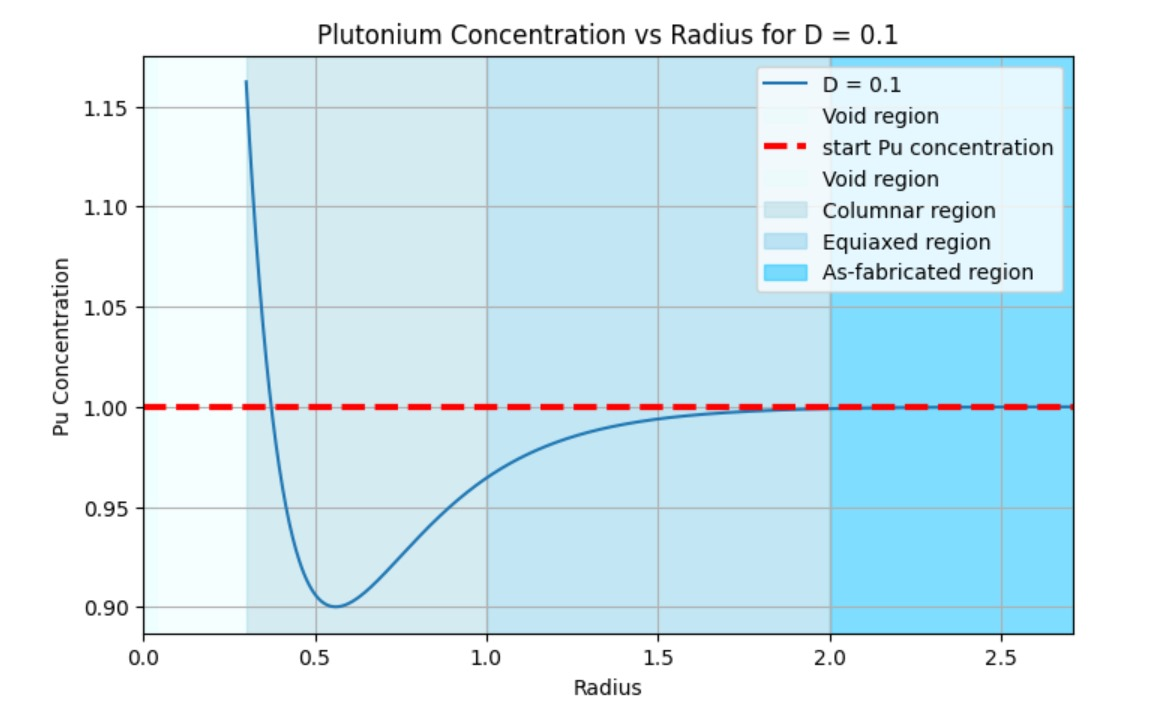
\includegraphics[width=0.8\textwidth]{Pu_redistribution_profile.jpg}
\caption{Radial distribution of Plutonium concentration (relative to the starting concentration) within the fuel structure.}
\label{fig:Pu_Profile}
\end{figure}

\subsubsection*{Impact on Design and Operation}
Plutonium enrichment in the central zone increases power density, leading to higher local temperatures. 
This effect must be managed to ensure the fuel remains below its melting point, particularly during extended operation. 
Redistribution can also worsen fuel swelling and impact cladding integrity, requiring careful consideration in the design phase.

\subsection{Helium Embrittlement}

Helium embrittlement occurs due to the accumulation of helium at grain boundaries in the cladding material, primarily produced by neutron-induced reactions such as $^{58}$Ni(n,$\alpha$)$^{55}$Fe. This leads to:

\begin{itemize}
    \item \textbf{Loss of ductility}: Making the material more brittle.
    \item \textbf{Crack formation}: Making the cladding more likely to crack.
    \item \textbf{Increased swelling}: Causing the material to expand under stress.
\end{itemize}

Helium concentrations after 1 and 2 years of operation are $67$~ppm and $122$~ppm, respectively. These values match those reported in the literature (\textit{Olander - Fundamentals Aspects of Nuclear Reactor Fuel Elements}).
A more accurate evaluation would require calculating helium per displacements-per-atom (ppm/DPA).


%%%%%%%%%%%%%%%%%%%%%%%%%%%%%%%%%%%%%%%%%%%%%%%%%%%%%%%%%%%%%%%%%%%%%%%%%%%%%%%%%%%%%%%%%%%%
\section{Critical Issues for Extended Operation}
With the selected dimensions, we extended the computation to simulate an uptime of 2 years instead of the initial 1-year design. The results demonstrate the performance and safety of the fuel pin under prolonged operational conditions:

\begin{itemize}
    \item {\color{green}\checkmark} \textbf{Maximum Fuel Temperature:} 2553.260 K (increased from 2480.096 K).
    \item \textbf{Maximum Cladding Temperature:} 912.696 K (unchanged).
    \item {\color{red}\texttimes} \textbf{Plenum Pressure:} 5.409 MPa (limit exceeded, increased from 2.792 MPa).
    \item \textbf{Maximum Instantaneous Cladding Plastic Strain:} 0.000\% (unchanged).
    \item \textbf{Maximum Cladding Volumetric Swelling:} 20.118\% (limit exceeded, increased significantly from 2.900\%).
    \item \textbf{Maximum Coolant Velocity:} 5.558 m/s (increased from 4.779 m/s).
    \item \textbf{Minimum Gap Thickness:} 367.927 microns (decreased from 386.495 microns).
    \item \textbf{Burnup:} 128.268 GWd/tHM (increased from 64.134 GWd/tHM).
    \item \textbf{Fuel Yielding Due to Swelling:} 8.979\% (increased from 4.489\%).
    \item \textbf{Time to Rupture:} 4.23 years (decreased significantly from 51.98 years).
\end{itemize}

\textbf{Comparison and Observations:}
\begin{itemize}
    \item The maximum fuel temperature increased slightly, indicating a higher thermal load on the fuel, likely due to increased burnup.
    \item The plenum pressure and cladding volumetric swelling both exceeded design limits, indicating that the fuel pin design is insufficient for extended irradiation cycles without adjustments.
    \item The burnup doubled, as expected
    \item The time to rupture decreased drastically from 51.98 years to 4.23 years, showing that thermal creep becomes a significant concern under these conditions.
    \item While the coolant velocity increased, it remained within acceptable operational ranges, highlighting that the thermal-hydraulic design is not a limiting factor in this scenario.
    \item The gap thickness decreased but the gap is still open, which guarantees no pellet-cladding interaction.
\end{itemize}

In summary, the significant rise in cladding swelling, plenum pressure, and reduced time to rupture indicate that this design requires further optimization to handle extended operation cycles safely.


%%%%%%%%%%%%%%%%%%%%%%%%%%%%%%%%%%%%%%%%%%%%%%%%%%%%%%%%%%%%%%%%%%%%%%%%%%%%%%%%%%%%%%%%%%%%
\section{Conclusions}
The finalized design meets all specified requirements for one year operation, ensuring safety and reliability. 
Conservative assumptions and thorough validation steps provided additional safety margins. 
The design demonstrates robustness under normal operating conditions but shows criticalities in extended operational conditions.

%%%%%%%%%%%%%%%%%%%%%%%%%%%%%%%%%%%%%%%%%%%%%%%%%%%%%%%%%%%%%%%%%%%%%%%%%%%%%%%%%%%%%%%%%%%%
\section*{Appendix}
All supporting code is available in the following repository: \href{https://github.com/simo-pagliu/NDT-Homeworks}{\textcolor{blue}{NDT-Homeworks Repository}}.
\begin{itemize}
    \item The final computation can be run from the \verb|Dimensioning.ipynb| Jupyter notebook, which calls functions from \verb|loop.py|.
    \item In-depth analysis and verification are found within \verb|Verification.ipynb|, which calls functions from \verb|functions.py|.
    \item \verb|genetic_algorithm.py| contains the implementation of the genetic algorithm.
    \item \verb|Useful Data.xlsx| contains cross-section data from the JANIS database.
    \item \verb|nuclei_func.py| contains a collection of functions to calculate nuclear properties.
\end{itemize}


%%%%%%%%%%%%%%%%%%%%%%%%%%%%%%%%%%%%%%%%%%%%%%%%%%%%%%%%%%%%%%%%%%%%%%%%%%%%%%%%%%%%%%%%%%%%
\end{document}
